%-----------------------------------------------------------------
% Shocktube 1D
%-----------------------------------------------------------------
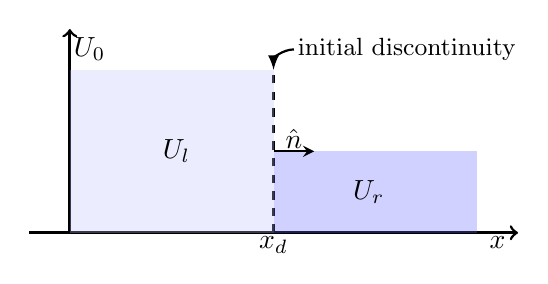
\begin{tikzpicture}[scale = {0.015\linewidth},inner sep = 1pt]

% create axis
%% \draw[->,line width=1pt] (0,0.5) |- (0.60,0) node[below]{$x$};
\draw[line width=1pt] (-0.5,0.45) node[right]{$\mbf{U}_0$}|-(0.55,0) node[below]{$x$};
\draw[->,line width=1pt] (0.55,0)--(0.6,0);
\draw[->,line width=1pt] (-0.5,0.45)--(-0.5,0.5);
\draw[line width=1pt] (-0,0)--(-0.6,0);  

% discontinuity
\draw[dashed,line width=1pt] (0,0) node[below]{$x_d$} -- (0,0.4); 
%% \draw[<-,line width=1pt] (-0.60,0) -- (0,0); 
\draw[-latex,thick](0.05,0.45)node[right]{\small initial discontinuity}
         to[out=180,in=90] (0,0.4);

% initial states
\fill[blue!25!,opacity=.3] (-0.5,0) rectangle (0,0.4);
\fill[blue!60!,opacity=.3] (0,0) rectangle (0.5,0.2);
\node[right] at (-0.28,0.2) {$\mbf{U}_l$};
\node[left] at (0.28,0.1) {$\mbf{U}_r$};


% normal
%% \draw[-stealth,thick] (0,0.25) -- (0.1,0.25); 
%% \node[] at (0.05,0.28) {$\hat{n}$};
\draw[-stealth,thick] (0,0.2) -- (0.1,0.2); 
\node[] at (0.05,0.23) {$\hat{n}$};

\end{tikzpicture}


%-----------------------------------------------------------------
% Shocktube 2D
%-----------------------------------------------------------------
%% \begin{tikzpicture}[scale = {0.015\linewidth},inner sep = 1pt]
%% % create axis
%% \draw[<->,line width=1pt] (0,0.6) node[right]{$y$} |- (1.1,0) node[below]{$x$};
%% %% \draw[<-,line width=1pt] (-0.75,0) -- (0,0); 

%% %% % normal
%% %% \draw[-stealth,thick] (0,0.25) -- (0.1,0.25); 
%% %% \node[] at (0.05,0.28) {$\hat{n}$};

%% % initial states
%% \draw[fill=blue!25!,opacity=.3] (0,0) -- (0,0.5) -- (1.0,0) -- cycle;
%% \draw[fill=blue!60!,opacity=.3] (0,0.5) -- (1.0,0.5) -- (1.0,0) -- cycle;
%% \node[right] at (0.2,0.15) {$\mbf{U}_0$};
%% \node[left] at (0.8,0.35) {$\mbf{U}_1$};

%% % discontinuity
%% \draw[line width = 1pt] (0,0.5) -- (1.0,0);
%% \draw[-latex,thick](0.2,0.55)node[right]{\small initial discontinuity}
%%          to[out=180,in=90] (0.1,0.45);

%% % normal
%% \draw[-stealth,thick] (0.5,0.25) -- (0.55,0.35); 
%% \node[] at (0.55,0.29) {$\hat{n}$};

%% \end{tikzpicture}
